% !TeX spellcheck = en_US

\documentclass[conference]{IEEEtran}
\usepackage{blindtext, cite, cleveref, float, graphicx, subcaption, url}



% correct bad hyphenation here
\hyphenation{op-tical net-works semi-conduc-tor}


\begin{document}
%
% paper title
% can use linebreaks \\ within to get better formatting as desired
\title{CiCTrie - C Implementation of CTrie}

% author names and affiliations
% use a multiple column layout for up to three different
% affiliations
\author{\IEEEauthorblockN{Daniel Solomon}
\IEEEauthorblockA{ID: \\
Email: DanielSolomon94.ds@gmail.com}
\and
\IEEEauthorblockN{Or Karni}
\IEEEauthorblockA{ID: \\
Email: orkarni@mail.tau.ac.il}}

% make the title area
\maketitle


\begin{abstract}
	We ported high-level memory managed data structure \textit{CTrie} to an unmanaged language \textit{C}, using \textit{hazard pointers} mechanism, while keeping the basic operations of the data structure. We compared our implementation against Scala's standard library \textit{TrieMap} (\textit{CTrie}) using similar tests as in the original article.
\end{abstract}

\begin{IEEEkeywords}
	CTrie, Hazard Pointers.
\end{IEEEkeywords}

\IEEEpeerreviewmaketitle

\section{Introduction}
		\textbf{CTrie}\cite{article}\cite{wiki-ctrie} (or concurrent hash-trie) is a concurrent \textit{thread-safe}, \textit{lock-free} implementation of a hash array mapped trie. This data structure is consists of \textit{key-value} pairs and it supports the following operations:
		\begin{itemize}
			\item \textbf{insert}: add a new \textit{(key, value)} pair.
			\item \textbf{remove}: remove a \textit{(key, value)} pair if it exists.
			\item \textbf{lookup}: find the \textit{value} (if any) for a specific \textit{key}. 
		\end{itemize}
		In addition the \textbf{CTrie} data structure has a \textit{snapshot} operation which is used to implement consistent \textit{iterators}. In fact \textbf{CTrie} is the first known concurrent data structure that supports \textit{O(1)}, \textit{atomic}, \textit{lock-free} snapshots.\\
		\textbf{CTrie} aspires to preserve the space-efficiency and the expected depth of hash tries by \textit{compressing} after removals, disposing of unnecessary nodes and thus keeping the depth reasonable.\\
		The \textbf{CTrie} implementation is based on single-word \textit{compare-and-swap} instructions. 

\section{Implementation}
	
	We wanted to give a simple interface for using \textit{CiCTrie}\cite{cictrie} which will be as close  as possible to object oriented programming, therefore we used \textit{Object Oriented C}; The user creates a \textit{ctrie\_t*} struct using a "constructor" \textit{create\_ctrie} and use its functions passing itself as a "self object" (such as: \texttt{ctrie->insert(\textbf{ctrie}, key, value)}). \\
	This way we could port easily the original \textit{Scala} code from the original paper \cite{article} and from the source code of the standard library itself \cite{ctrie-scala-source-code}. \\
	In addition, \textit{CiCTrie} supports only int keys and values, although if needed it can support any data structure as \textit{keys} and \textit{values}, without managing their memory. It can be implemented easily, if one will pass a \textit{hash} function when calling \texttt{ctrie\_create} and all keys and values will be \texttt{void*}.
	
\subsection{Basic Operations}
	All basic operations were implemented; \texttt{insert, lookup, remove, clean, compress, to\_contracted and clean\_parent}; Where the latter one was implemented but it is not used since this optimization does not improve any performance at all.
	
\subsection{Memory Reclamation}
	\textit{Hazard pointers} are a mechanism which aims to solve the ABA and safe memory reclamation problems\cite{hazard}\cite{wiki-hazard}. Each thread maintains a list of \textit{hazard pointers} to resources it currently uses. This list usually has a fixed size and is kept small. A used resource may not be freed or modified.\\
	In the worst case scenario a specific thread holds 4 different pointers that were dynamically allocated, for example:
	When reaching a \textit{TNode} we must clean it, the thread acquired 2 hazard pointers for the parent \textit{INode} and its \textit{MainNode} of type \textit{CNode} and in \texttt{compress} function the thread acquires another 2 hazard pointers for each \textit{INode} child and its \textit{MainNode}. \\
	In our implementation, each thread has a list of 6 \textit{hazard pointers} in total - 4 "ctrie" \textit{hazard pointers} and 2 "list" \textit{hazard pointers}. The list \textit{hazard pointers} is used for traverse a \textit{LNode} and for using "temporary" \textit{hazard pointers} in compress (hazard pointers which can be shortly overridden). \\
	We implemented two lighter versions using 5 \textit{hazard pointers} in total\cite{5-hp-cictrie} for each thread (4 \textit{hazard pointers} for \textit{LNode} and "ctrie" \textit{hazard pointers} and 1 "temporary" \textit{hazard pointer}) and another version using 4 \textit{hazard pointers} only (minimal as mentioned)\cite{4-hp-cictrie}. This implementation is dividing the \textit{hazard pointers} into 2 pairs. One pair is used for the CAS while the other is used for preparing the new node to be inserted. In each call, the current pair is determined by the level oddity - so it alternates. When inserting or removing a \textit{SNode} or a \textit{LNode}, the pair of the current inode and main node is the CAS pair, and the other 2 \textit{hazard pointers} can be overridden freely. When cleaning a \textit{TNode}, the parent \textit{INode} and it's \textit{MainNode} are the CAS pair, and the other 2 \textit{hazard pointers} can be overridden freely. \\
	Comparing both lighter versions to the 6 \textit{hazard pointers} version we got better performance for the greedy 6 \textit{hazard pointers} implementation (See \textit{BENCHMARKING} section). \\\\
	Before accessing anything, a thread must first place a \textit{hazard pointer} to ensure no one will free the desired memory. However, \textit{hazard pointers} by themselves don't guarantee success. For example, if a thread reaches an \textit{INode} and wishes to continue down to it's \textit{MainNode}, it reads the pointer to the \textit{MainNode}, places a \textit{hazard pointer} and then accesses the node. But what if between the read and the placement of the \textit{hazard pointer}, another thread changes the \textit{CTrie} and frees the \textit{MainNode}? The original thread would place a \textit{hazard pointer} on an invalid address and wouldn't know it's already freed. To solve this problem, we added a \textit{marked} field to \textit{INode}, \textit{LNode} and \textit{CNode}. The marked field indicates that this node has been removed from the \textit{CTrie} and is scheduled for freeing. In places where a race might occur, the accessing thread must validate it's state after placing a \textit{hazard pointer}. In the example above, the thread must validate that:
	\begin{enumerate}
		\item The \textit{INode} isn't marked.
		\item The \textit{Inode} still points to the expected \textit{MainNode}.		
	\end{enumerate}
	If the race occurs the thread must \textit{RESTART} its operation. Any node that points to another node should have a \textit{marked} field for race detection, the only nodes that points to others are \textit{INode}, \textit{LNode} and \textit{CNode}. \\
	Since \textit{marked} property must be accessible for any thread and must be up-to-date any time, after marking a node (or multiple nodes), a \textit{FENCE} operation is invoked. \\
	Each thread holds a fixed size free list. The size is determined by the number of threads times number of \textit{hazard pointers} that is used in the implementation (For example in our 6 \textit{hazard pointers} implementation, with 4 threads, each thread has a free list of size 24). This size is needed in order to make sure no "dead locks" will happen, since when the free list is full, a thread must free at list one member of the list before continuing its operations, therefore when getting to the free phase, it must be guaranteed that at least one member of the free list does not occur in any \textit{hazard pointers} lists of the other threads.
	
\subsection{Snapshot}
	The \textit{CTrie} data structure support a \textit{O(1)}, \textit{atomic}, \textit{lock-free} \textit{snapshot} operation. This feature is implemented by replacing the CAS operation with a GCAS operation. The GCAS simulates an atomic DCAS, which doesn't exist natively on most machines. Each \textit{INode} is assigned to a generation. A snapshot increases the root \textit{INode}'s generation number. Each thread that encounters an \textit{INode} of and older generation than the root it has seen at the start of the operation, it copies the inode and it's main node, replaces the old inode with the copy and continues operating on the copy. This way, the \textit{INode}'s of the original generation stay unchanged and thus the snapshot isn't affected. 
	With the concern of memory management, the snapshot procedure is a bit more complicated. In our implementation, each \textit{MainNode} also has a generation number. When a thread removes a node of an older generation from the trie, it doesn't free it because it "belongs" to a snapshot. However, freeing a snapshot is a complicated action. Because of the lazy copying of the nodes, it is unknown whether a node in the snapshot is still in the actual new generation \textit{CTrie}, and so it mustn't be freed. Because of this, and the rarity of snapshot operations, which are less useful in \textit{C} than they are in \textit{Scala} because there are no iterators, we've decided that a snapshot cannot be freed, which creates an acceptable memory leak.
	The snapshot implementation\cite{snapshot-cictrie} is implemented in a different branch because of it's inherent difference from the "clean" implementation.

\section{Benchmarking}

\subsection{Experiments}
	We performed experimental measurements on a machine with 44 cores and 2 hyper-threads per core, 88 threads total. \textit{Scala} version 2.12.3, JDK 8 and sbt version 1.0.0 configuration was used. \\
	Since we are using integers as keys, there will be no \textit{LNode}s at all, because a hash collision will occur only if the keys collide. Therefore, we changed the \textit{hash} function to: $hash(x) = x / 10$ (both in \textit{CiCTrie} and in Scala) in order to create collisions of different keys. \\
	Each benchmark was run for 20 iterations with 1, 2, 4, 8, 16, 32, 44, 66 and 88 threads per iteration. We measured \textit{insert}, \textit{lookup} and \textit{remove} operations by generating a sample of 2 million numbers between 0 and 5 million. Each run starts from an empty \textit{ctrie} instance, inserts the whole sample, lookups for each key and then removes all keys. Insertions, lookups and removes were time measured separately. All operations were divided equally by all available threads (for example, in configuration of 4 threads, each thread runs 500,000 inserts, lookups and removes). The same benchmark was performed for our \textit{C} implementation and for the \textit{Scala} implementation (See Fig. \ref{fig:isolated_operations}). The \textit{Garbage Collector} was invoked between \textit{Scala} operations and wasn't included in the measured time. \\
	The first 6 benchmarks don't include the \textit{Scala} and compare the 4 and 5 \textit{hazard pointers} C implementations with the 6 \textit{hazard pointers} C implementation (See Fig. \ref{fig:4_hazard_pointers_implementations}, \ref{fig:5_hazard_pointers_implementations}) \\
	The final 3 benchmarks are called 90-9-1, 80-15-5, 60-30-10 consist of inserts, lookups and removes invoked in the respective ratio. 2 million operations on keys between 0 and 5 million are created and shuffled (See Fig. \ref{fig:heterogeneous_operations}).

\subsection{Results}
	As is clearly visible, the \textit{Scala} implementation's performance is better than the \textit{C} implementation. We attribute this performance difference to \textit{Scala} and \textit{JVM} optimizations. However, it should be noted that the \textit{C} implementation consumes much less memory (around two times less memory). Also, the gap between the implementation grows smaller as the thread count increases (except for inserts). This happens because the \textit{Scala} implementation doesn't benefit very much from more than 32 threads, while the \textit{C} implementation does, so it might stay improvable with more threads while \textit{Scala} will not. \\
	One anomaly we've noticed is a considerable slowdown between 1 and 2 threads. This phenomenon happened only on the benchmarking machine and we don't know it's cause.\\
	Another interesting property is the unbridged gap between the implementations in the insert benchmark. A constant gap of about 1 second remained between the implementations even when the thread count increased. We've profiled the \textit{C} implementation's performance in order to improve the performance. There wasn't an abnormal amounts of \textit{RESTART}'s. The memory management and \textit{hazard pointers}'s time consumption is not significant enough to cause the performance difference. When using a profiling tool, \textit{perf}\cite{wiki-perf}, no suspiciously time consuming routine has arose. It appeared that simple memory reads and writes took most of the time. \\
	As for the 5 \textit{hazard pointers} implementation, we've had better performance with the 6 \textit{hazard pointers} implementation. The overhead of the \textit{hazard pointers} check in \texttt{scan} is probably lower than the \texttt{hp\_list} management overhead (less \textit{hazard pointers} require more sophisticated management). \\
	Notice that both in \textit{Scala}'s and \textit{C}'s results, except to few number of threads the longest run and shortest run are very close to each other. The standard deviation for insert and lookup is smaller than the remove's most likely because the probability to be \textit{RESTART}ed in remove is bigger (\textit{CAS} races and \textit{TNodes}) [All numbers are in nano-seconds] (See Table \ref{scala_table} and Table \ref{c_table}).   
	
	\begin{table}[H]
		\caption{Scala - Variance/Min/Max}
		\label{scala_table}
		\begin{center}
			\scalebox{0.8}{
				\begin{tabular}{c | c | c | c | c}
					$\textbf{Threads}$ & $ \textbf{Operation} $ & $ \textbf{Variance} $ & $ \textbf{Min} $ & $ \textbf{Max} $ \\ \hline
					1  & insert & 8.46e+14 & 1565517868  & 1667691751  \\
					2  & insert & 2.86e+15 & 863842838   & 1051936962  \\
					4  & insert & 1.02e+15 & 467942163   & 561266596   \\
					8  & insert & 3.52e+14 & 260197276   & 322273773   \\
					16 & insert & 6.46e+13 & 156279438   & 180283871   \\
					32 & insert & 1.18e+13 & 113353978   & 126449294   \\
					44 & insert & 7.25e+12 & 101493346   & 115129822   \\
					66 & insert & 1.45e+13 & 93313236    & 110542513   \\
					88 & insert & 1.93e+13 & 99354941    & 115267184   \\
					1  & lookup & 1.30e+16 & 1588477005  & 1967220906  \\
					2  & lookup & 1.68e+14 & 831415860   & 892782333   \\
					4  & lookup & 5.38e+13 & 415750029   & 443283217   \\
					8  & lookup & 2.57e+13 & 213251410   & 235864087   \\
					16 & lookup & 2.62e+12 & 109709780   & 115369755   \\
					32 & lookup & 1.41e+11 & 57900029    & 59351450    \\
					44 & lookup & 7.08e+13 & 44471729    & 84596094    \\
					66 & lookup & 2.14e+13 & 33457898    & 47158422    \\
					88 & lookup & 5.95e+12 & 38603780    & 48496281    \\
					1  & remove & 3.42e+15 & 2341652734  & 2558173043  \\
					2  & remove & 1.27e+15 & 1293776067  & 1417738473  \\
					4  & remove & 9.26e+14 & 648160830   & 768317981   \\
					8  & remove & 4.94e+14 & 360462934   & 445821495   \\
					16 & remove & 1.37e+14 & 199690864   & 250172785   \\
					32 & remove & 8.03e+13 & 121204469   & 162866851   \\
					44 & remove & 2.74e+13 & 119500160   & 136728323   \\
					66 & remove & 1.20e+13 & 101274083   & 114641203   \\
					88 & remove & 1.28e+14 & 104149189   & 153960945   \\
				\end{tabular}
			}	
		\end{center}
	\end{table}
	
	\begin{table}[H]
		\caption{C - Variance/Min/Max}
		\label{c_table}
		\begin{center}
			\scalebox{0.8}{
				\begin{tabular}{c | c | c | c | c}
					$\textbf{Threads}$ & $ \textbf{Operation} $ & $ \textbf{Variance} $ & $ \textbf{Min} $ & $ \textbf{Max} $ \\ \hline
					1  & insert & 9.15e+14 & 3373524969 & 3476078641   \\
					2  & insert & 3.26e+17 & 3299984707 & 5128231007   \\
					4  & insert & 1.21e+17 & 1894273634 & 3016384274   \\
					8  & insert & 2.15e+16 & 1165826762 & 1650697393   \\
					16 & insert & 5.55e+15 & 923573895  & 1228303155   \\
					32 & insert & 2.76e+15 & 837945372  & 1021218363   \\
					44 & insert & 1.21e+15 & 815866044  & 963055571    \\
					66 & insert & 3.33e+14 & 805731658  & 874692640    \\
					88 & insert & 2.40e+14 & 805209930  & 867190137    \\
					1  & lookup & 2.09e+15 & 2554887913 & 2702243292   \\
					2  & lookup & 1.53e+18 & 1557068892 & 5305724781   \\
					4  & lookup & 7.64e+17 & 771727951  & 3518754762   \\
					8  & lookup & 2.21e+17 & 388718763  & 1884118200   \\
					16 & lookup & 9.10e+16 & 192139601  & 1287779436   \\
					32 & lookup & 5.24e+16 & 99774608   & 829316269    \\
					44 & lookup & 3.68e+16 & 74222433   & 766205832    \\
					66 & lookup & 1.81e+16 & 52388882   & 395748260    \\
					88 & lookup & 4.09e+15 & 59396617   & 244680555    \\
					1  & remove & 6.59e+15 & 7349148262 & 7619081115   \\
					2  & remove & 1.83e+18 & 6318573302 & 10773737757  \\
					4  & remove & 8.22e+17 & 3483085900 & 6357503854   \\
					8  & remove & 2.70e+17 & 1848544432 & 3557135601   \\
					16 & remove & 1.34e+17 & 946780919  & 2378249792   \\
					32 & remove & 9.41e+16 & 545096904  & 1531001275   \\
					44 & remove & 9.61e+16 & 424420636  & 1535618365   \\
					66 & remove & 2.41e+16 & 290965405  & 733644623    \\
					88 & remove & 1.82e+15 & 228875070  & 365224656    \\
				\end{tabular}
			}	
		\end{center}
	\end{table}
	
	
	\begin{figure}
		\begin{subfigure}{.5\textwidth}
			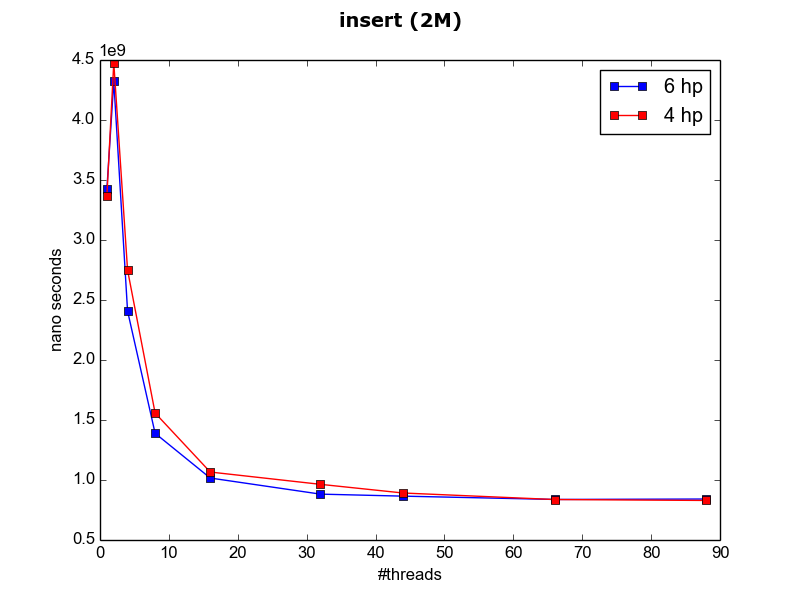
\includegraphics[width=0.45\paperwidth]{hp_comapre/insert_2M_4hp.png}
			\label{fig:4hp_insert}			
		\end{subfigure}
		\begin{subfigure}{.5\textwidth}
			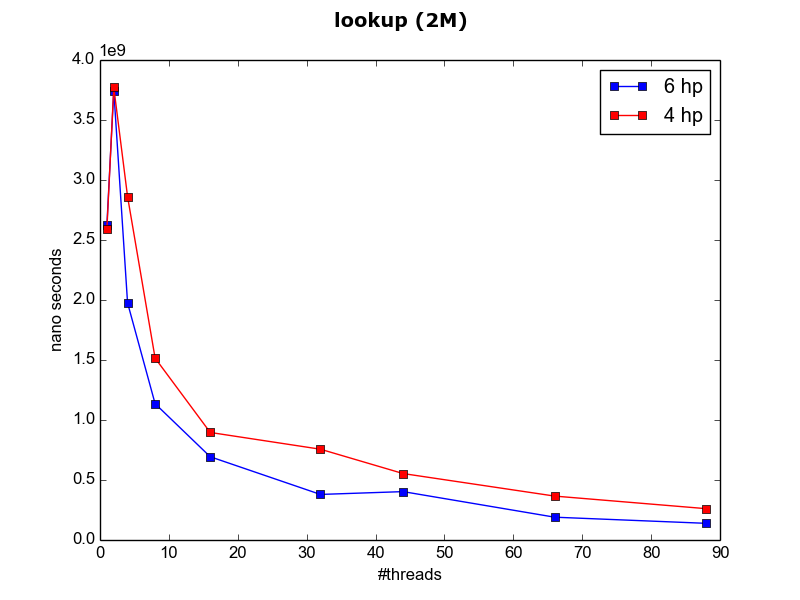
\includegraphics[width=0.45\paperwidth]{hp_comapre/lookup_2M_4hp.png}	
			\label{fig:4hp_lookup}
		\end{subfigure}
		\begin{subfigure}{.5\textwidth}
			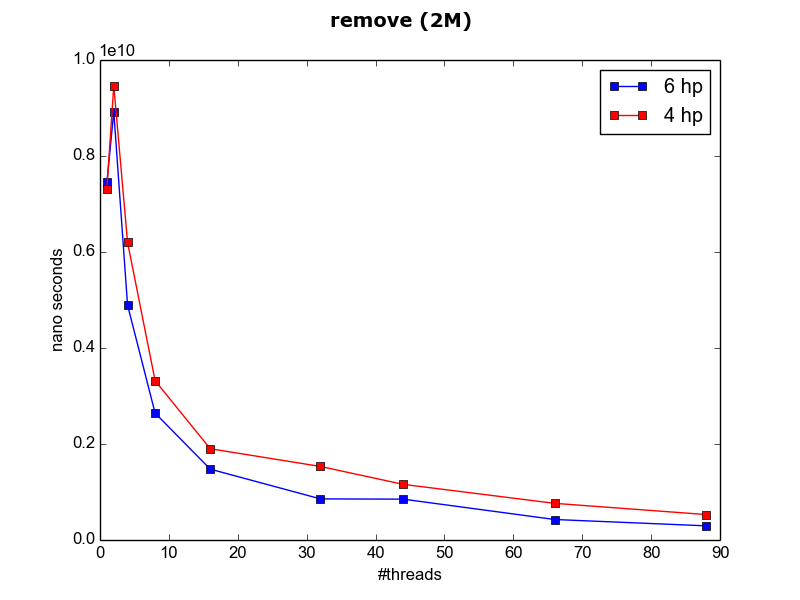
\includegraphics[width=0.45\paperwidth]{hp_comapre/remove_2M_4hp.png}
			\label{fig:4hp_remove}
		\end{subfigure}
		\caption{hazard pointers implementations (6 vs 4)}
		\label{fig:4_hazard_pointers_implementations}
	\end{figure}
	\begin{figure}
		\begin{subfigure}{.5\textwidth}
			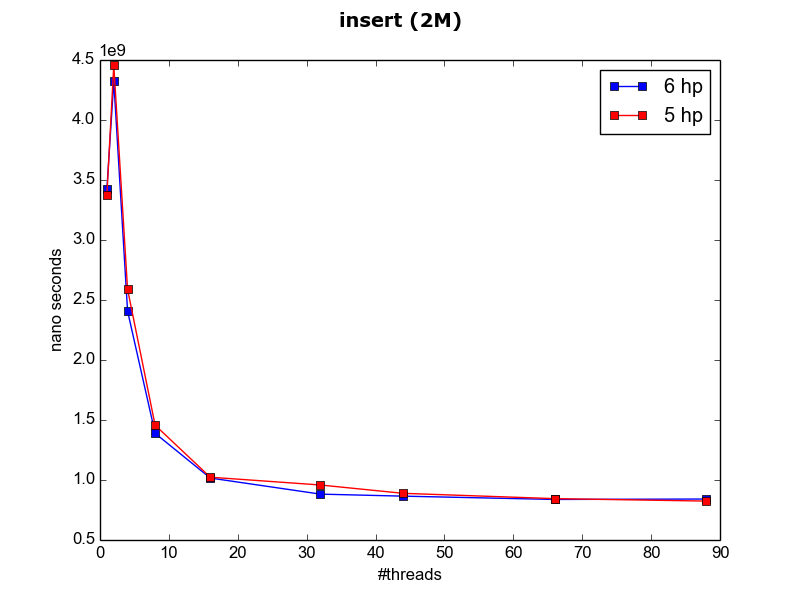
\includegraphics[width=0.45\paperwidth]{hp_comapre/insert_2M_5hp.png}
			\label{fig:5hp_insert}			
		\end{subfigure}
		\begin{subfigure}{.5\textwidth}
			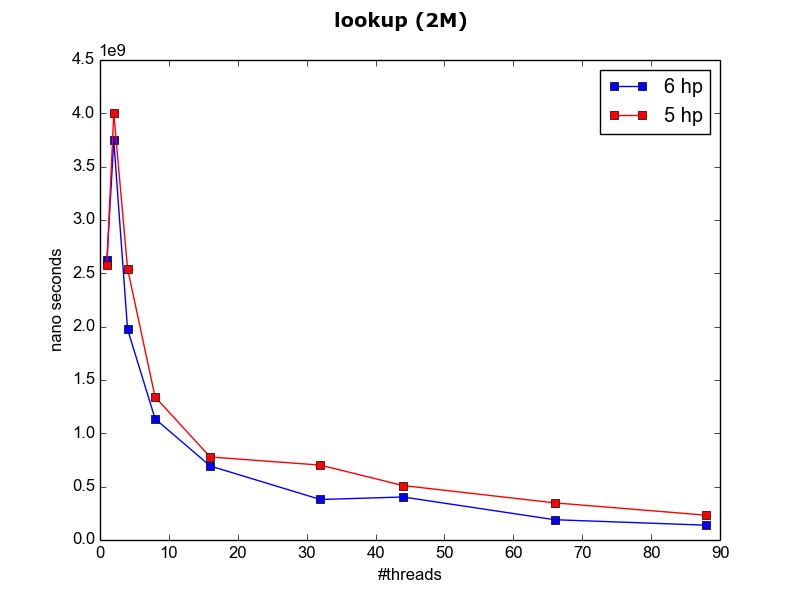
\includegraphics[width=0.45\paperwidth]{hp_comapre/lookup_2M_5hp.png}	
			\label{fig:5hp_lookup}
		\end{subfigure}
		\begin{subfigure}{.5\textwidth}
			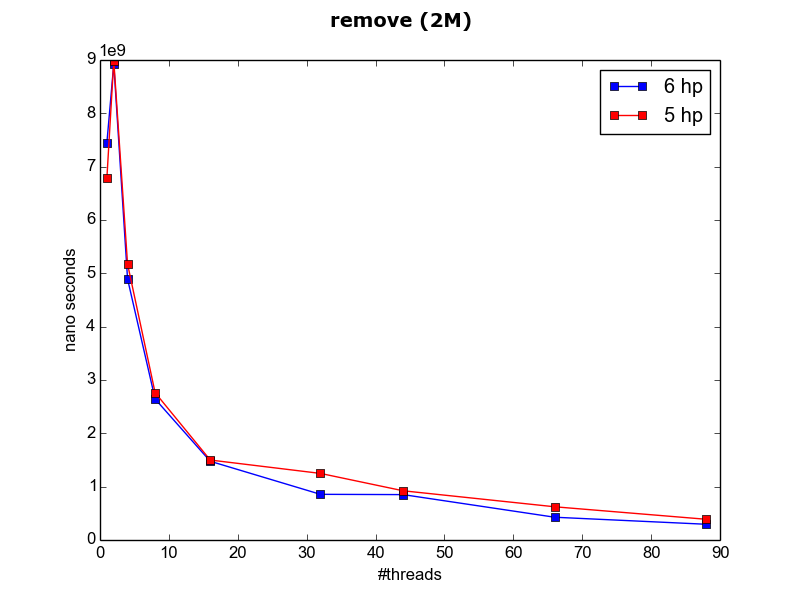
\includegraphics[width=0.45\paperwidth]{hp_comapre/remove_2M_5hp.png}
			\label{fig:5hp_remove}
		\end{subfigure}
		\caption{hazard pointers implementations (6 vs 5)}
		\label{fig:5_hazard_pointers_implementations}
	\end{figure}

	\begin{figure}
		\begin{subfigure}{.5\textwidth}
			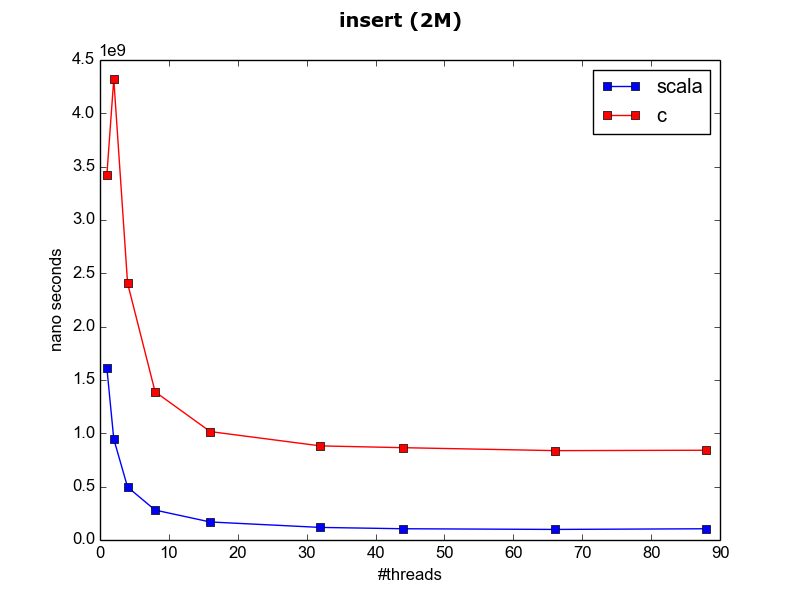
\includegraphics[width=0.45\paperwidth]{vs_scala/insert_2M.png}
			\label{fig:c_vs_scala_insert}			
		\end{subfigure}
		\begin{subfigure}{.5\textwidth}
			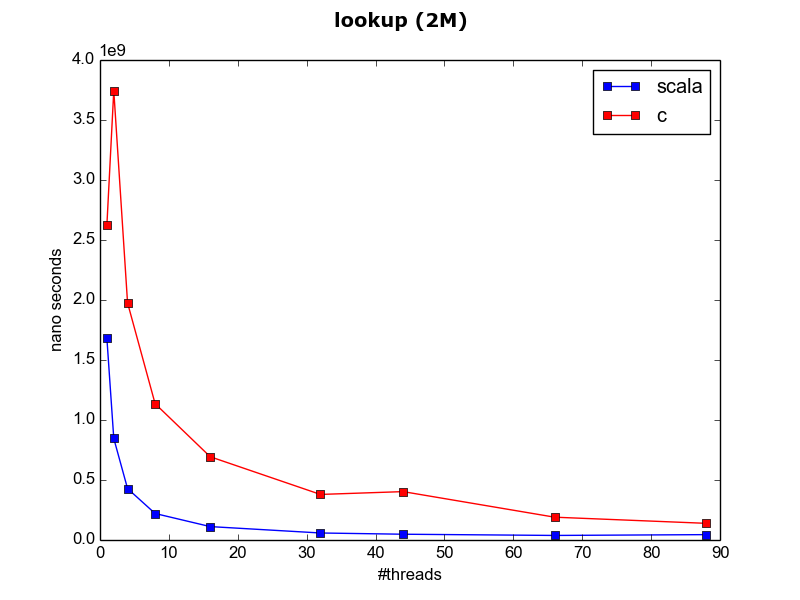
\includegraphics[width=0.45\paperwidth]{vs_scala/lookup_2M.png}	
			\label{fig:c_vs_scala_lookup}
		\end{subfigure}
		\begin{subfigure}{.5\textwidth}
			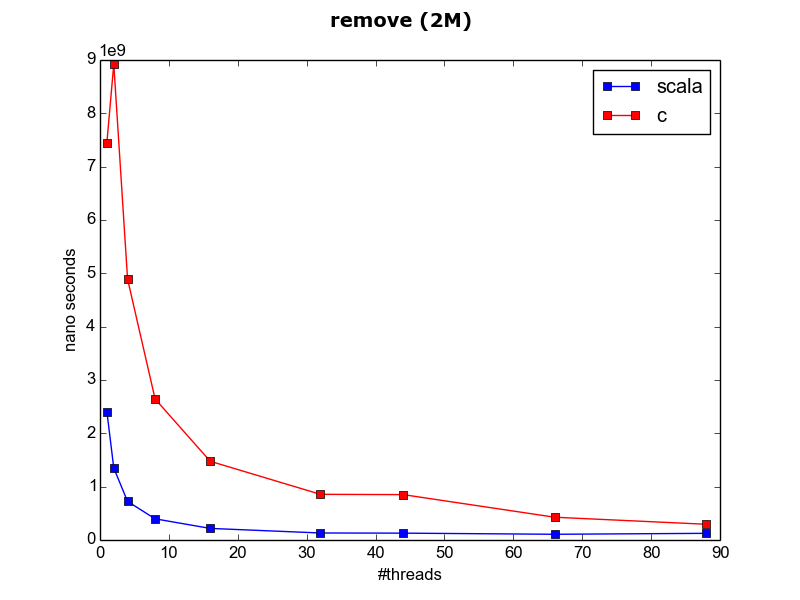
\includegraphics[width=0.45\paperwidth]{vs_scala/remove_2M.png}
			\label{fig:c_vs_scala_remove}
		\end{subfigure}
		\caption{C vs Scala implementations (isolated operations)}
		\label{fig:isolated_operations}
	\end{figure}	

	\begin{figure}
		\begin{subfigure}{.5\textwidth}
			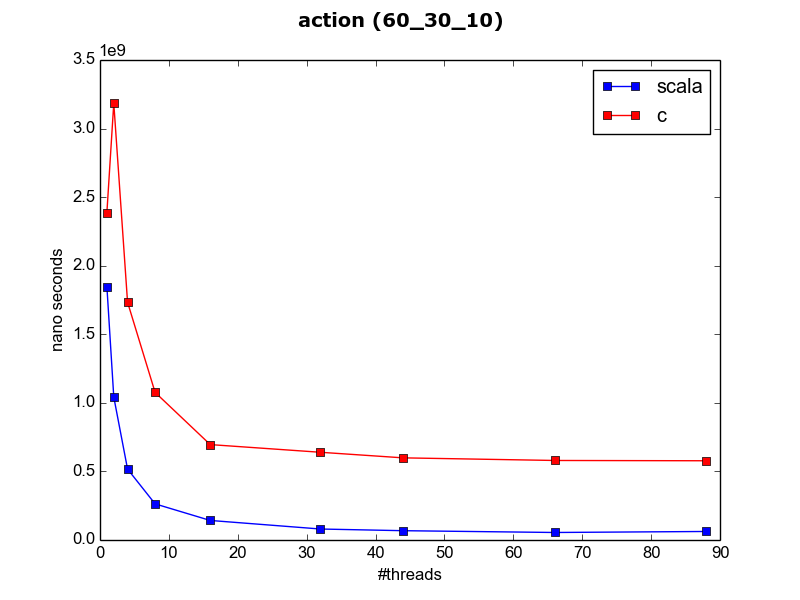
\includegraphics[width=0.45\paperwidth]{vs_scala/action_60_30_10.png}
			\label{fig:c_vs_scala_60_30_10}
		\end{subfigure}
		\begin{subfigure}{.5\textwidth}
			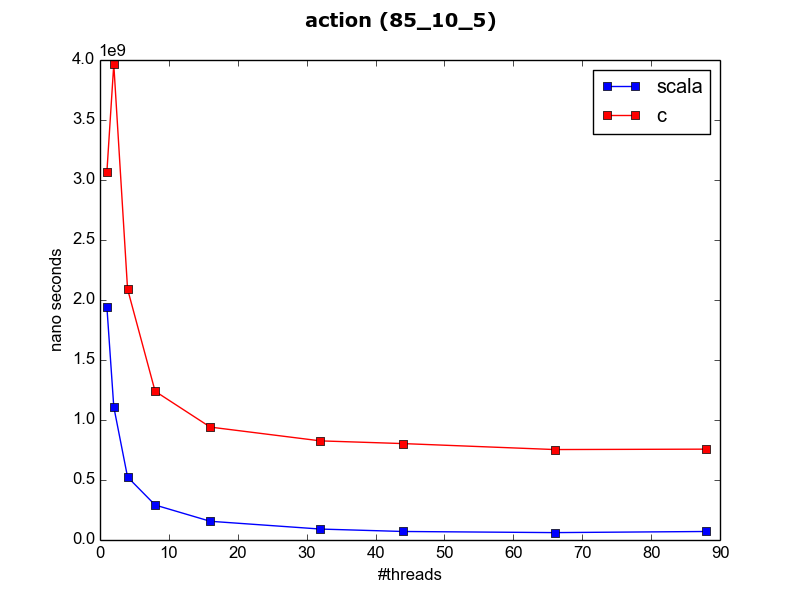
\includegraphics[width=0.45\paperwidth]{vs_scala/action_85_10_5.png}
			\label{fig:c_vs_scala_85_10_5}
		\end{subfigure}
		\begin{subfigure}{.5\textwidth}
			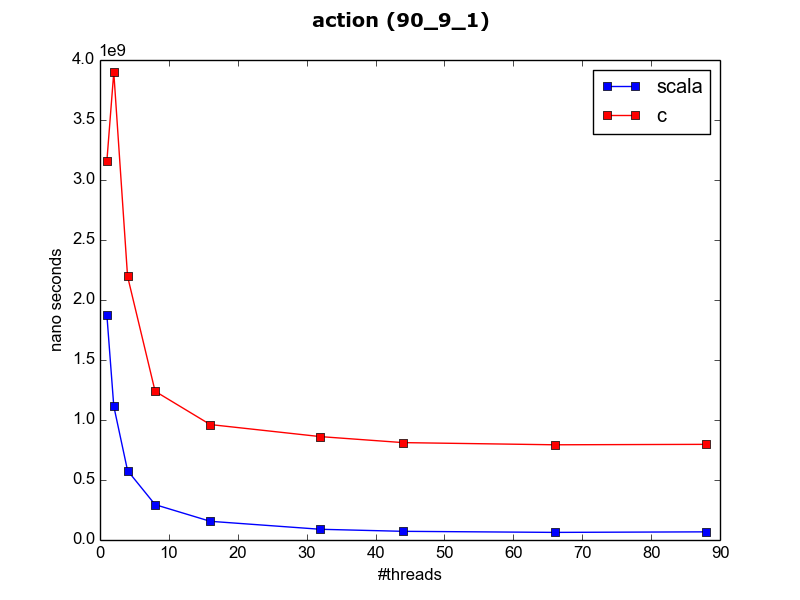
\includegraphics[width=0.45\paperwidth]{vs_scala/action_90_9_1.png}
			\label{fig:c_vs_scala_90_9_1}
		\end{subfigure}
		\caption{C vs Scala implementations (heterogeneous operations)}
		\label{fig:heterogeneous_operations}
	\end{figure}	


\begin{thebibliography}{1}
	\bibitem{article} Original article representing \textbf{CTrie} - \url{https://axel22.github.io/resources/docs/ctries-snapshot.pdf}. 
	\bibitem{wiki-ctrie} \textbf{CTrie} wikipedia reference - \url{https://en.wikipedia.org/wiki/Ctrie}.
	\bibitem{cictrie} The \textbf{CiCTrie} on GitHub -
	\url{https://github.com/DanielSolomon/CiCTrie}
	\bibitem{ctrie-scala-source-code} TrieMap Scala source code - \url{https://www.scala-lang.org/api/current/scala/collection/concurrent/TrieMap.html}.
	\bibitem{hazard} Original article of hazard pointers - 
	\url{https://www.research.ibm.com/people/m/michael/ieeetpds-2004.pdf}
	\bibitem{wiki-hazard} Hazard pointers wikipedia reference - \url{https://en.wikipedia.org/wiki/Hazard_pointer}.
	\bibitem{5-hp-cictrie} The \textbf{CiCTrie} with 5 hazard pointers -
	\url{https://github.com/DanielSolomon/CiCTrie/tree/71f08706f92d5023823fd08de9300281022b8f98}
	\bibitem{4-hp-cictrie} The \textbf{CiCTrie} with 4 hazard pointers -
	\url{https://github.com/DanielSolomon/CiCTrie/tree/4hp}
	\bibitem{snapshot-cictrie} The \textbf{CiCTrie} with snapshot -
	\url{https://github.com/DanielSolomon/CiCTrie/tree/snapshot}
	\bibitem{wiki-perf} Perf wiki-  \url{https://perf.wiki.kernel.org/index.php/Main_Page}.
	
\end{thebibliography}

% that's all folks
\end{document}


